\documentclass[12pt]{article}

\usepackage{report}

\usepackage[utf8]{inputenc} % allow utf-8 input
\usepackage[T1]{fontenc}    % use 8-bit T1 fonts
\usepackage[colorlinks=true, linkcolor=black, citecolor=blue, urlcolor=blue]{hyperref}       % hyperlinks
\usepackage{url}            % simple URL typesetting
\usepackage{booktabs}       % professional-quality tables
\usepackage{amsfonts}       % blackboard math symbols
\usepackage{nicefrac}       % compact symbols for 1/2, etc.
\usepackage{microtype}      % microtypography
\usepackage{lipsum}		% Can be removed after putting your text content
\usepackage{graphicx}
\usepackage{natbib}
\usepackage{doi}
\usepackage{listings}
\usepackage{xcolor}
\usepackage{float}
\setcitestyle{aysep={,}}



\title{Project Step 2}

\author{Ulises Espinoza-Gonzalez and Jack Stolpman\\
\AND\\
\AND
\AND
\AND
\AND
	CS.3339 Computer Architecture\\
\AND
	Texas State University\\
}

% Uncomment to remove the date
\date{October 29, 2024}

% Uncomment to override  the `A preprint' in the header
\renewcommand{\headeright}{Project Step 2 - Tomato}
\renewcommand{\undertitle}{Group Tomato}
\renewcommand{\shorttitle}{}

\definecolor{codegreen}{rgb}{0,0.6,0}
\definecolor{codegray}{rgb}{0.5,0.5,0.5}
\definecolor{codepurple}{rgb}{0.58,0,0.82}
\definecolor{backcolour}{rgb}{0.95,0.95,0.92}

\lstdefinestyle{mystyle}{
    backgroundcolor=\color{backcolour},   
    commentstyle=\color{codegreen},
    keywordstyle=\color{magenta},
    numberstyle=\tiny\color{codegray},
    stringstyle=\color{codepurple},
    basicstyle=\ttfamily\footnotesize,
    breakatwhitespace=false,         
    breaklines=true,                 
    captionpos=b,                    
    keepspaces=true,                 
    numbers=left,                    
    numbersep=5pt,                  
    showspaces=false,                
    showstringspaces=false,
    showtabs=false,                  
    tabsize=2
}

\lstset{style=mystyle}


\begin{document}
\maketitle

\newpage
%\tableofcontents
\thispagestyle{empty}


\newpage
\setcounter{page}{1}
\section{Introduction}
Digital logic and circuits are an essential part of understanding the hardware components of any electronic device. Hardware descriptive languages such as Verilog, introduce us to the process of designing a new computer circuit from scratch. In this first section of our project, we will be utilizing 1-bit Not, Nand, Nor, and 1x4-bit input / 1x4-bit output shift circuits to generate simulation waveforms. Some goals that we as a group share is to improve our understanding of the methodology of designing new computer circuits from scratch. We also wish to familiarize ourselves with the Verilog programming language, which is new to us. 

\section{Verilog Code}
\label{sec:headings}

In this section, we are going to go over the circuits and then the Verilog code for each one with the test modules.





\section{And Circuit}
The And circuit takes two inputs, A and B, with an output X. In order for the output of this gate to be 1, both inputs must also be 1. This logic gate works well with operations that require all conditions to be met simultaneously.
\lstinputlisting[language=Verilog]{Verilog/and_gate_tb.v}

To test the And circuit, we have created two registers, A and B, as well as a wire X. This way we can take two inputs at a time and test each possible input for the circuit. If it's working correctly, X should be equal to 1 for all inputs only when both A and B are equal to 1.
\lstinputlisting[language=Verilog]{Verilog/and_gate.v}

\begin{figure}[h]
    \centering
    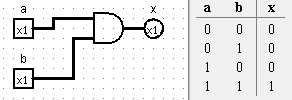
\includegraphics[width = 1.0\textwidth]{figs/andGate.png}
    \caption{And truth table and gate}
    \label{fig:enter-label}
\end{figure}


\subsection{Waveform Tests}

The last section we will showcase the waveforms created using our testbenches for each circuit we coded in Verilog. We used GTKWave to create these waveforms.

\newpage




\section{Nand Circuit}
The Nand circuit, similarly to the And circuit, takes two inputs- A and B, with an output X. This output will only shoot back a 1 assuming that both A and B are not equal to 1, hence the Nand (Not and) logic gate.
\lstinputlisting[language=Verilog]{Verilog/nand_gate_tb.v}

To test the Nand circuit, we have created two registers, A and B, as well as a wire X. This way we are able to take two inputs at a time and test each possible input for the circuit. If it's working correctly, X should be equal to 1 for all inputs except when both A and B are equal to 1. This gate is often used in circuits as a building block as it can be combined to create other logic gates.
\lstinputlisting[language=Verilog]{Verilog/nand_gate.v}

\begin{figure}[h]
    \centering
    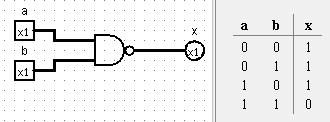
\includegraphics[width = 1.0\textwidth]{figs/Nand CircuitTruth.png}
    \caption{Nand truth table and gate}
    \label{fig:enter-label}
\end{figure}

\newpage

\subsection{Waveform Tests}

The last section we will showcase the waveforms created using our testbenches for each circuit we coded in Verilog. We used GTKWave to create these waveforms.





\section{Or Circuit}
The Or circuit takes two inputs, A and B, with an output X. This output will only shoot back a 1 assuming that either A, B. or both are equal to 1. If both a and b are 0, the output will also be 0. This gate is often used in circuits were an output is required when at least one condition is true.
\lstinputlisting[language=Verilog]{Verilog/or_gate_tb.v}

To test the Or circuit, we have created two registers, A and B, as well as a wire X. This way we are able to take two inputs at a time and test each possible input for the circuit. If it's working correctly, X should be equal to 1 whenever a or b (or both) are equal to 1.
\lstinputlisting[language=Verilog]{Verilog/or_gate.v}

\begin{figure}[h]
    \centering
    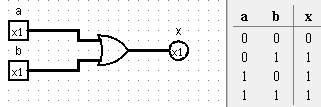
\includegraphics[width = 1.0\textwidth]{figs/or.png}
    \caption{Or truth table and gate}
    \label{fig:enter-label}
\end{figure}



\subsection{Waveform Tests}

The last section we will showcase the waveforms created using our testbenches for each circuit we coded in Verilog. We used GTKWave to create these waveforms.







\section{Nor Circuit}
The Nor circuit takes two inputs, A and B, with an output X. This output will only shoot back a 1 assuming that both A and B are equal to 0, hence the Nor logic gate. For the output to return a high value, both inputs need to be low. This gate is often used in circuits where the output is true when all inputs are false.
\lstinputlisting[language=Verilog]{Verilog/nor_gate_tb.v}

To test the Nor circuit, we have created two registers, A and B, as well as a wire X. This way we are able to take two inputs at a time and test each possible input for the circuit. If it's working correctly, X should be equal to 1 for all inputs except when both A and B are equal to 0. 
\lstinputlisting[language=Verilog]{Verilog/nor_gate.v}

\begin{figure}[h]
    \centering
    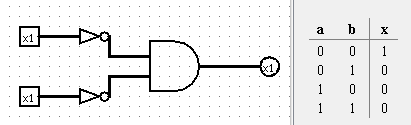
\includegraphics[width = 1.0\textwidth]{figs/Nor CircuitTruth.png}
    \caption{Nor truth table and gate}
    \label{fig:enter-label}
\end{figure}

\newpage

\subsection{Waveform Tests}

The last section we will showcase the waveforms created using our testbenches for each circuit we coded in Verilog. We used GTKWave to create these waveforms.







\section{Xor Circuit}
The Xor circuit takes two inputs, A and B, with an output X. This output will only shoot back a 1 assuming that only one of the inputs is 1. if A and B are different (A = 1, B = 0), then the output will be 1. 
\lstinputlisting[language=Verilog]{Verilog/xor_gate_tb.v}

To test the Xor circuit, we have created two registers, A and B, as well as a wire X. This way we are able to take two inputs at a time and test each possible input for the circuit. If it's working correctly, X should be equal to 1 only when one of the inputs is equal to 1. This gate is often used in circuits that require distinguishing between inputs.
\lstinputlisting[language=Verilog]{Verilog/xor_gate.v}

\begin{figure}[h]
    \centering
    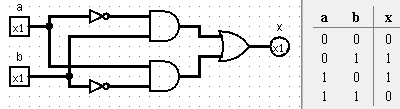
\includegraphics[width = 1.0\textwidth]{figs/xor.png}
    \caption{Xor truth table and gate}
    \label{fig:enter-label}
\end{figure}


\subsection{Waveform Tests}

The last section we will showcase the waveforms created using our testbenches for each circuit we coded in Verilog. We used GTKWave to create these waveforms.







\section{Xnor Circuit}
The Xnor circuit takes two inputs, A and B, with an output X. This output will only shoot back a 1 assuming that both A and B are the same value (A = 1, B = 1 || A = 0, B = 0). If the value for A is different from that of B, then the output will be 0.
\lstinputlisting[language=Verilog]{Verilog/xnor_gate_tb.v}

To test the Xnor circuit, we have created two registers, A and B, as well as a wire X. This way we can take two inputs at a time and test each possible input for the circuit. If it's working correctly, X should be equal to 1 only when A and B have the same value. This gate is used in circuits where we need the output to be true when both inputs match.
\lstinputlisting[language=Verilog]{Verilog/xnor_gate.v}

\begin{figure}[h]
    \centering
    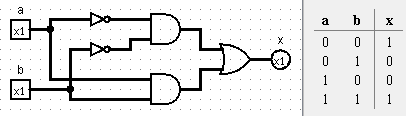
\includegraphics[width = 1.0\textwidth]{figs/xnorgate.png}
    \caption{Xnor truth table and gate}
    \label{fig:enter-label}
\end{figure}

\newpage

\subsection{Waveform Tests}

The last section we will showcase the waveforms created using our testbenches for each circuit we coded in Verilog. We used GTKWave to create these waveforms.









\section{Not Circuit}
The Not circuit takes two inputs: A and B.The Not gate will revert the value inputted. If the value of A is 1, then the value of B will be 0 and vice versa.
\lstinputlisting[language=Verilog]{Verilog/not_gate_tb.v}

To test the Not circuit, we have created two registers, A and B. This way we can take two inputs at a time and test each possible input for the circuit. If it's working correctly, A should be equal to 1 whenever B is equal to 0.
\lstinputlisting[language=Verilog]{Verilog/not_gate.v}

\begin{figure}[h]
    \centering
    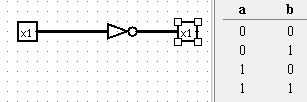
\includegraphics[width = 1.0\textwidth]{figs/Not CircuitTruth.png}
    \caption{Not truth table and gate}
    \label{fig:enter-label}
\end{figure}

\newpage



\subsection{Waveform Tests}

The last section we will showcase the waveforms created using our testbenches for each circuit we coded in Verilog. We used GTKWave to create these waveforms.








\section{2x4-bit input Circuit}
The 4 bit input circuit takes two inputs, fourin and fourout. We create a shift input. 
\lstinputlisting[language=Verilog]{Verilog/four_bit_input_tb.v}
To test this 4 bit circuit, we create a register that takes in a 4 bit value. This value works alongside the clock which when executed using the @posedge and the clock signal goes from high to low, the input will be transfered into the output.

\lstinputlisting[language=Verilog]{Verilog/four_bit_input.v}



\subsection{Waveform Tests}

The last section we will showcase the waveforms created using our testbenches for each circuit we coded in Verilog. We used GTKWave to create these waveforms.






\section{2x4-bit output Shift Circuit}
The 4 bit input circuit takes two inputs, datain and dataout. We use a clock/ reset and create a shift input in order to determine the shift direction (high = 1 = right, low = 0 = left).  On the rising edge of the reset, we set the output to 4'b0000 (0 in verilog) which clears the shift register. While this process is happening, if the shift is high, the data is shifted right by 1 bit and when the shift is low, the data is shifted left by 1 bit.

\lstinputlisting[language=Verilog]{Verilog/four_bit_shift_circuit_tb.v}

To test the 4bit shift circuit, we have created two registers, A and B, as well as a wire X. We also create a.
\lstinputlisting[language=Verilog]{Verilog/four_bit_shift_circuit.v}



\subsection{Waveform Tests}

The last section we will showcase the waveforms created using our testbenches for each circuit we coded in Verilog. We used GTKWave to create these waveforms.










\section{Addition}
The addition module takes in two inputs - A and B - which are both 4-bit. These represent the numbers that will be added. We then create the sum output which is the 4-bit result of the addition. the carry in is a single bit representing any carry coming in from previous calculations. Due to us adding 4-bit values, we create a 5 bit wire called addition result which accounts for any overflow we may encounter. 
\lstinputlisting[language=Verilog]{Verilog/addition_tb.v}

To test the addition of the 4-bit values, we assign the sum of A and B and the carry in to our 5 bit variable. Once assigned, the 5-bit wire stores the 4 least significant bits and stores them into our sum output. We finally assign the overflow bit to the carry out.
\lstinputlisting[language=Verilog]{Verilog/addition.v}







\subsection{Waveform Tests}

The last section we will showcase the waveforms created using our testbenches for each circuit we coded in Verilog. We used GTKWave to create these waveforms.






\section{Subtraction}
The subtraction module takes in two inputs - A and B - which are both 4-bit. These represent the numbers that will be added. We then create the difference output which is the 4-bit result of the subtraction. the carry in is a single bit that acts as a borrow input in our calculations. Due to us subtracting 4-bit values, we create a 5 bit wire called subtraction result which accounts for any overflow we may encounter. 
\lstinputlisting[language=Verilog]{Verilog/subtraction_tb.v}

To test the subtraction of the 4-bit values, we assign the difference of A and B and the carry in to our 5 bit variable. Once assigned, the 5-bit wire stores the 4 least significant bits which the difference output later recieves. The carry out will hold the borrow bit only if A < B.
\lstinputlisting[language=Verilog]{Verilog/subtraction.v}




\subsection{Waveform Tests}

The last section we will showcase the waveforms created using our testbenches for each circuit we coded in Verilog. We used GTKWave to create these waveforms










\section{Multiplication}
The multiplication module takes in two 4-bit inputs - A and B. The inputs represent the numbers that will be multiplied. We also create an output called product in order to store the value of the multiplication.
\lstinputlisting[language=Verilog]{Verilog/multiplication_tb.v}

In order to multiply the two 4-bit values, we have to ensure that our product can handle any overflow. We can achieve this by making the product an 8-bit value. This is because the multiplication of two 4-bit values may produce up to an 8-bit value. We then simply assign the multiplication of A and B to the product variable.
\lstinputlisting[language=Verilog]{Verilog/multiplication.v}





\subsection{Waveform Tests}

The last section we will showcase the waveforms created using our testbenches for each circuit we coded in Verilog. We used GTKWave to create these waveforms.







\section{Division}
The division module takes in two 4-bit inputs - A and B. The inputs represent the numbers that will be divided. We also create two 4-bit outputs which are the quotient and remainder. These will be used to store their respective values.
\lstinputlisting[language=Verilog]{Verilog/division_tb.v}

In order to divide the two 4-bit values, we simply assign the division of A and B to the quotient variable. We then use modulo in order to determine if there is a remainder and then assign the value to its corresponding output. We also use the modulo as a check to see if b is equal to 0. We do this in order to ensure that we aren't dividing A by 0.
\lstinputlisting[language=Verilog]{Verilog/division.v}




\subsection{Waveform Tests}

The last section we will showcase the waveforms created using our testbenches for each circuit we coded in Verilog. We used GTKWave to create these waveforms.







\section{Conclusion}

In conclusion, we successfully created and tested various circuits using Verilog and GTKWave. Learning how to code in Verilog, at least for our purposes, was relatively simple with few difficulties. Using GTKWave was also fairly intuitive. The most difficulty our group has had so far was most likely creating this report in LaTeX, as we have some trouble with coding certain formatting as well as issues with figures floating around the document. Creating these logic circuits from scratch allowed us to work on the basic logic gates (NOT, NAND, NOR) that are so critical to all electronics. The use of Verilog and GTKWave works as a stepping stone to furthering our engineering careers and building on our knowledge of both the software and hardware components of electronics.


\newpage

\section{Waveforms}



\subsection{And Circuit Waveform}

At 0 s, we can see that both A and B are 0, so the output is 0
\begin{figure}[h]
    \centering
    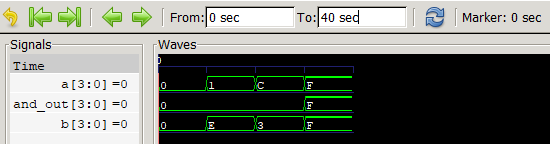
\includegraphics[width = 1.0\textwidth]{figs/And0.png}
    \caption{And Circuit with marker at 0s}
    \label{fig:enter-label}
\end{figure}

At 10 s, A is 1 and B is E, so the output is 0
\begin{figure}[h]
    \centering
    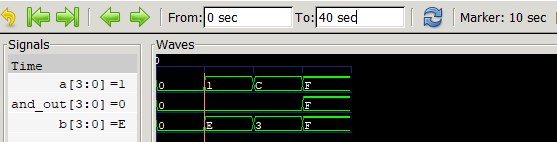
\includegraphics[width = 1.0\textwidth]{figs/And10.png}
    \caption{And Circuit with marker at 10s}
    \label{fig:enter-label}
\end{figure}


At 20 s, A is 1 and B is E, so the output is 0
\begin{figure}[h]
    \centering
    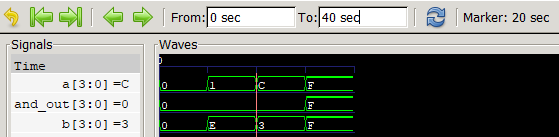
\includegraphics[width = 1.0\textwidth]{figs/And20.png}
    \caption{And Circuit with marker at 20s}
    \label{fig:enter-label}
\end{figure}


\newpage


At 30 s, A is F and B is F, so the output is F
\begin{figure}[h]
    \centering
    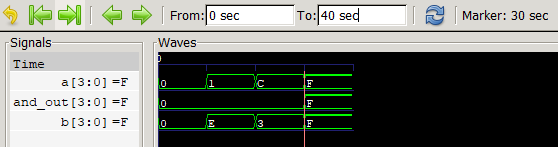
\includegraphics[width = 1.0\textwidth]{figs/And30.png}
    \caption{And Circuit with marker at 30s}
    \label{fig:enter-label}
\end{figure}




\subsection{Nand Circuit Waveform}

At 0 s, we can see that both A and B are 0, so the output is F
\begin{figure}[h]
    \centering
    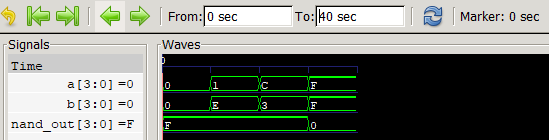
\includegraphics[width = 1.0\textwidth]{figs/Nand0.png}
    \caption{Nand Circuit with marker at 0s}
    \label{fig:enter-label}
\end{figure}

At 10 s, A is 1 and B is E, so the output is F
\begin{figure}[h]
    \centering
    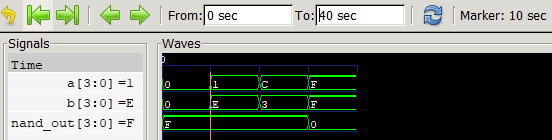
\includegraphics[width = 1.0\textwidth]{figs/Nand10.png}
    \caption{Nand Circuit with marker at 10s}
    \label{fig:enter-label}
\end{figure}

\newpage

At 20 s, A is C and B is 3, so the output is F
\begin{figure}[h]
    \centering
    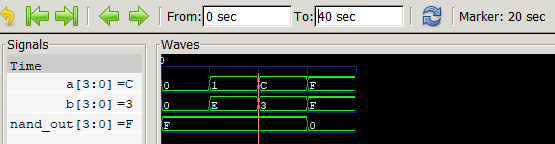
\includegraphics[width = 1.0\textwidth]{figs/Nand20.png}
    \caption{Nand Circuit with marker at 20s}
    \label{fig:enter-label}
\end{figure}



At 30 s, A is F and B is F, so the output is 0
\begin{figure}[h]
    \centering
    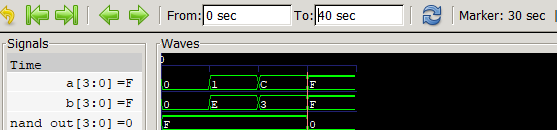
\includegraphics[width = 1.0\textwidth]{figs/Nand30.png}
    \caption{Nand Circuit with marker at 30s}
    \label{fig:enter-label}
\end{figure}


\newpage



\subsection{Or Circuit Waveform}

At 0 s, we can see that both A and B are 0, so the output is 0
\begin{figure}[h]
    \centering
    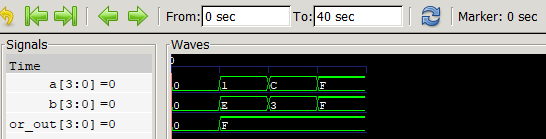
\includegraphics[width = 1.0\textwidth]{figs/Or0.png}
    \caption{Or Circuit with marker at 0s}
    \label{fig:enter-label}
\end{figure}


At 10 s, we can see that A is 1 and B is E, so the output is F
\begin{figure}[h]
    \centering
    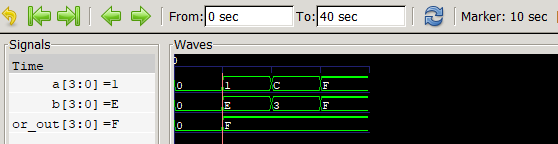
\includegraphics[width = 1.0\textwidth]{figs/Or10.png}
    \caption{Or Circuit with marker at 10s}
    \label{fig:enter-label}
\end{figure}

At 20 s, A is C and B is 3, so the output is F
\begin{figure}[h]
    \centering
    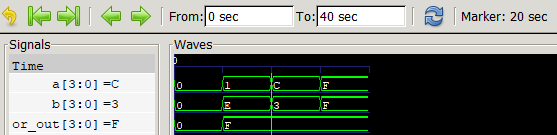
\includegraphics[width = 1.0\textwidth]{figs/Or20.png}
    \caption{Or Circuit with marker at 20s}
    \label{fig:enter-label}
\end{figure}

\newpage

At 30 s, A is F and B is F, so the output is F
\begin{figure}[h]
    \centering
    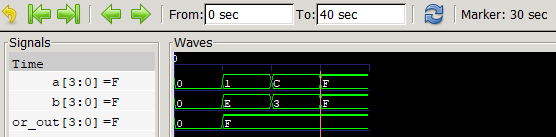
\includegraphics[width = 1.0\textwidth]{figs/Or30.png}
    \caption{Or Circuit with marker at 30s}
    \label{fig:enter-label}
\end{figure}


\subsection{Nor Circuit Waveform}

At 0 s, we can see that both A and B are 0, so the output is F
\begin{figure}[h]
    \centering
    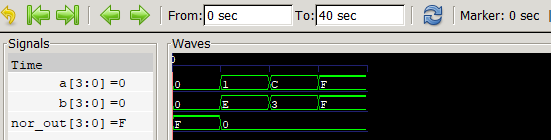
\includegraphics[width = 1.0\textwidth]{figs/Nor0.png}
    \caption{Nor Circuit with marker at 0s}
    \label{fig:enter-label}
\end{figure}


At 10 s, we can see that A is 1 and B is E, so the output is 0
\begin{figure}[h]
    \centering
    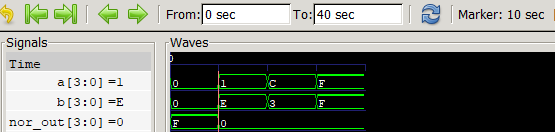
\includegraphics[width = 1.0\textwidth]{figs/Nor10.png}
    \caption{Nor Circuit with marker at 10s}
    \label{fig:enter-label}
\end{figure}

At 20 s, A is C and B is 3, so the output is 0
\begin{figure}[h]
    \centering
    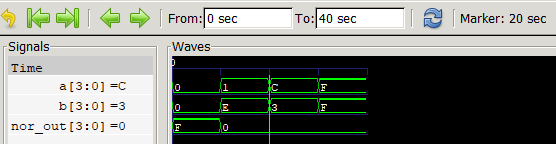
\includegraphics[width = 1.0\textwidth]{figs/Nor20.png}
    \caption{Nor Circuit with marker at 20s}
    \label{fig:enter-label}
\end{figure}

\newpage

At 30 s, A is F and B is F, so X is 0
\begin{figure}[h]
    \centering
    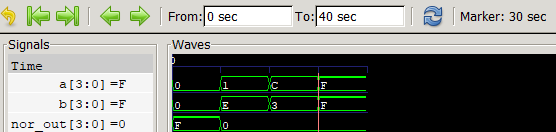
\includegraphics[width = 1.0\textwidth]{figs/Nor30.png}
    \caption{Nor Circuit with marker at 30s}
    \label{fig:enter-label}
\end{figure}




\subsection{Xor Circuit Waveform}

At 0 s, we can see that both A and B are 0, so the output is 0
\begin{figure}[h]
    \centering
    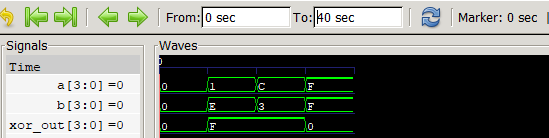
\includegraphics[width = 1.0\textwidth]{figs/Xor0.png}
    \caption{Xor Circuit with marker at 0s}
    \label{fig:enter-label}
\end{figure}

\newpage

At 10 s, we can see that A is 1 and B is E, so the output is F
\begin{figure}[h]
    \centering
    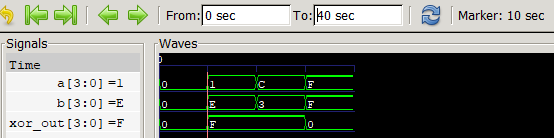
\includegraphics[width = 1.0\textwidth]{figs/Xor10.png}
    \caption{Xor Circuit with marker at 10s}
    \label{fig:enter-label}
\end{figure}

At 20 s, A is C and B is 3, so the output is F
\begin{figure}[h]
    \centering
    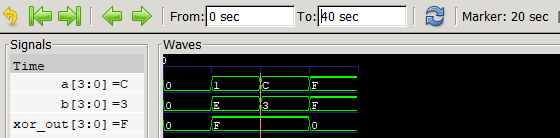
\includegraphics[width = 1.0\textwidth]{figs/Xor20.png}
    \caption{Xor Circuit with marker at 20s}
    \label{fig:enter-label}
\end{figure}


At 30 s, A is F and B is F, so the output is 0
\begin{figure}[h]
    \centering
    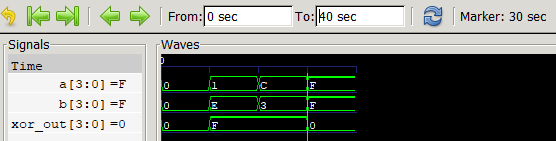
\includegraphics[width = 1.0\textwidth]{figs/Xor30.png}
    \caption{Xor Circuit with marker at 30s}
    \label{fig:enter-label}
\end{figure}

\newpage


\subsection{Xnor Circuit Waveform}

At 0 s, we can see that both A and B are 0, so the output is F
\begin{figure}[h]
    \centering
    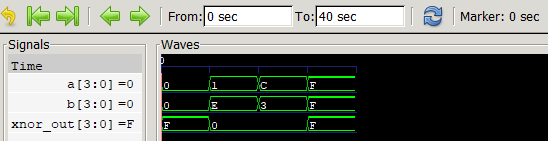
\includegraphics[width = 1.0\textwidth]{figs/Xnor0.png}
    \caption{Xnor Circuit with marker at 0s}
    \label{fig:enter-label}
\end{figure}


At 10 s, we can see that A is 1 and B is E, so the output is 0
\begin{figure}[h]
    \centering
    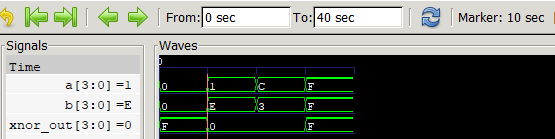
\includegraphics[width = 1.0\textwidth]{figs/Xnor10.png}
    \caption{Xnor Circuit with marker at 10s}
    \label{fig:enter-label}
\end{figure}

At 20 s, A is C and B is 3, so the output is 0
\begin{figure}[h]
    \centering
    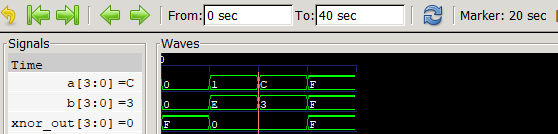
\includegraphics[width = 1.0\textwidth]{figs/Xnor20.png}
    \caption{Xnor Circuit with marker at 20s}
    \label{fig:enter-label}
\end{figure}

\newpage

At 30 s, A is F and B is F, so the output is F
\begin{figure}[h]
    \centering
    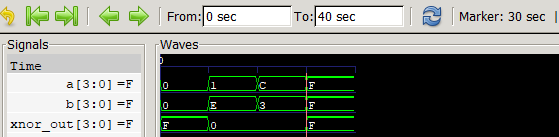
\includegraphics[width = 1.0\textwidth]{figs/Xnor30.png}
    \caption{Xnor Circuit with marker at 30s}
    \label{fig:enter-label}
\end{figure}



\subsection{Not Circuit Waveform}

At 0 s, we can see that both A and B are 0, so the not A is F and the not B is F
\begin{figure}[h]
    \centering
    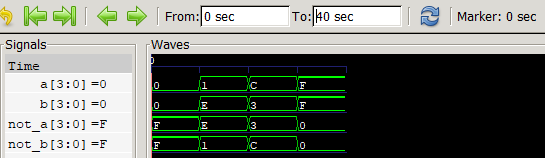
\includegraphics[width = 1.0\textwidth]{figs/Not0.png}
    \caption{Not Circuit with marker at 0s}
    \label{fig:enter-label}
\end{figure}

\newpage

At 10 s, A is 1 and B is E, so the not A is E and the not B is 1
\begin{figure}[h]
    \centering
    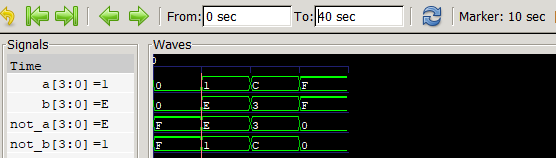
\includegraphics[width = 1.0\textwidth]{figs/Not10.png}
    \caption{Not Circuit with marker at 10s}
    \label{fig:enter-label}
\end{figure}


At 20 s, A is C and B is 3, so the not A is 3 and the not B is C
\begin{figure}[h]
    \centering
    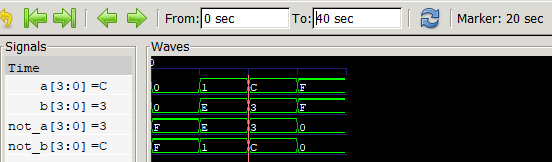
\includegraphics[width = 1.0\textwidth]{figs/Not20.png}
    \caption{Not Circuit with marker at 20s}
    \label{fig:enter-label}
\end{figure}

At 30 s, both A and B are F, so the not A is 0 and the not B is 0
\begin{figure}[h]
    \centering
    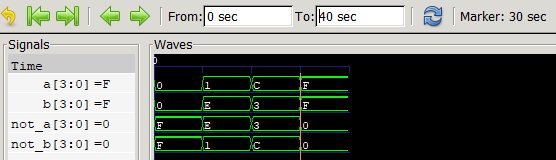
\includegraphics[width = 1.0\textwidth]{figs/Not30.png}
    \caption{Not Circuit with marker at 30s}
    \label{fig:enter-label}
\end{figure}




\subsection{2x4-bit input Circuit Waveform}

At 0 s, we can see that four in1 is0X and four in2 is 0, so the output for four out1 is X and four out2 is X
\begin{figure}[h]
    \centering
    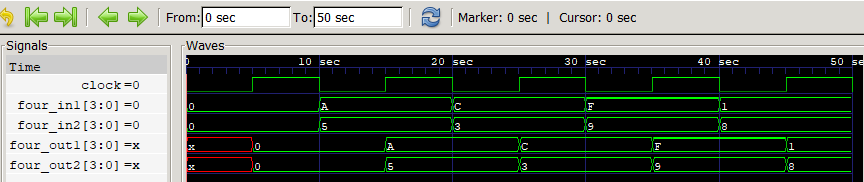
\includegraphics[width = 1.0\textwidth]{figs/Input0.png}
    \caption{2x4-bit input Circuit with marker at 0s}
    \label{fig:enter-label}
\end{figure}


At 10 s, we can see that four in1 is A and four in2 is 5, so the output for four out1 is 0 and four out2 is 0
\begin{figure}[h]
    \centering
    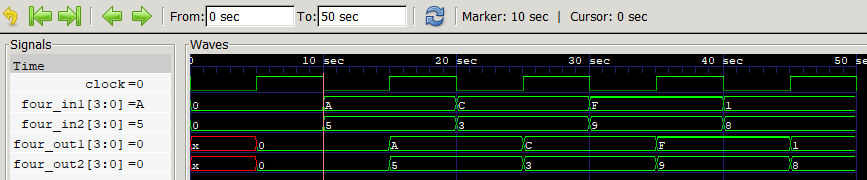
\includegraphics[width = 1.0\textwidth]{figs/Input10.png}
    \caption{2x4-bit input Circuit with marker at 10s}
    \label{fig:enter-label}
\end{figure}


At 20 s, we can see that four in1 is C and four in2 is 3, so the output for four out1 is A and four out2 is 5
\begin{figure}[h]
    \centering
    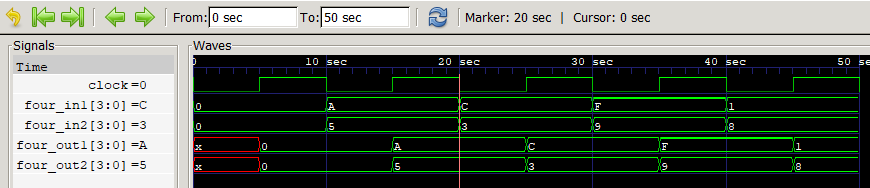
\includegraphics[width = 1.0\textwidth]{figs/Input20.png}
    \caption{2x4-bit input Circuit with marker at 20s}
    \label{fig:enter-label}
\end{figure}

\newpage

At 30 s, we can see that four in1 is F and four in2 is 9, so the output for four out1 is C and four out2 is 3
\begin{figure}[h]
    \centering
    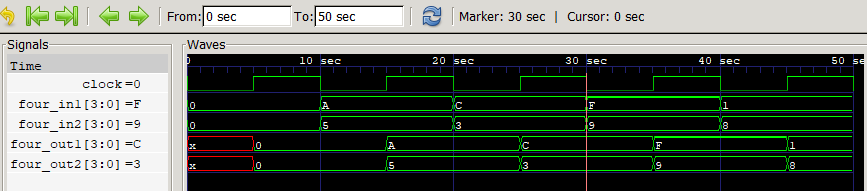
\includegraphics[width = 1.0\textwidth]{figs/Input30.png}
    \caption{2x4-bit input Circuit with marker at 30s}
    \label{fig:enter-label}
\end{figure}

At 40 s, we can see that four in1 is 1 and four in2 is 8, so the output for four out1 is F and four out2 is 9
\begin{figure}[h]
    \centering
    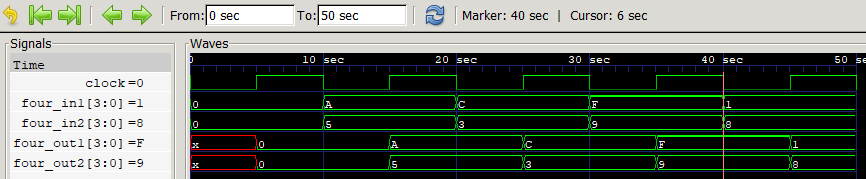
\includegraphics[width = 1.0\textwidth]{figs/Input40.png}
    \caption{2x4-bit input Circuit with marker at 40s}
    \label{fig:enter-label}
\end{figure}

At 50 s, we can see that four in1 is 1 and four in2 is 8, so the output for four out1 is 1 and four out2 is 8
\begin{figure}[h]
    \centering
    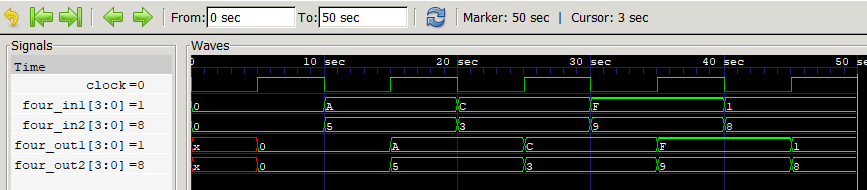
\includegraphics[width = 1.0\textwidth]{figs/Input50.png}
    \caption{2x4-bit input Circuit with marker at 50s}
    \label{fig:enter-label}
\end{figure}

\newpage

\subsection{2x4-bit output Shift Circuit Waveform}

At 0 s, we can see that data in1 is 0 and data in2 is 0, so that means that data out1 is 0 and data out2 is 0
\begin{figure}[h]
    \centering
    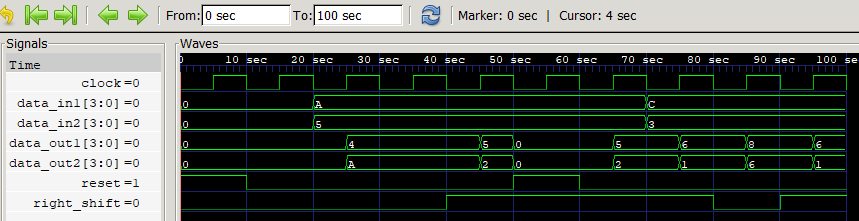
\includegraphics[width = 1.0\textwidth]{figs/Shift0.png}
    \caption{2x4-bit output Shift Circuit with marker at 0s}
    \label{fig:enter-label}
\end{figure}


At 10 s,we can see that data in1 is 0 and data in2 is 0, so that means that data out1 is 0 and data out2 is 0
\begin{figure}[h]
    \centering
    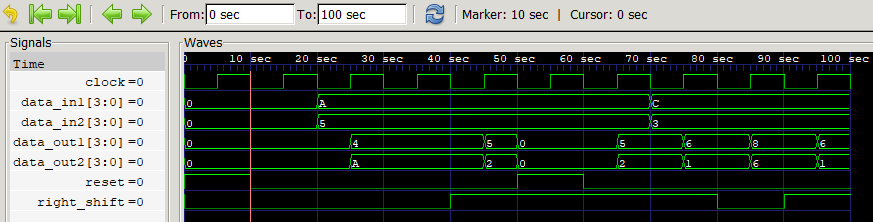
\includegraphics[width = 1.0\textwidth]{figs/Shift10.png}
    \caption{2x4-bit output Shift Circuit with marker at 10s}
    \label{fig:enter-label}
\end{figure}

\newpage

At 20 s, we can see that data in1 is A and data in2 is 5, so that means that data out1 is 0 and data out2 is 0
\begin{figure}[h]
    \centering
    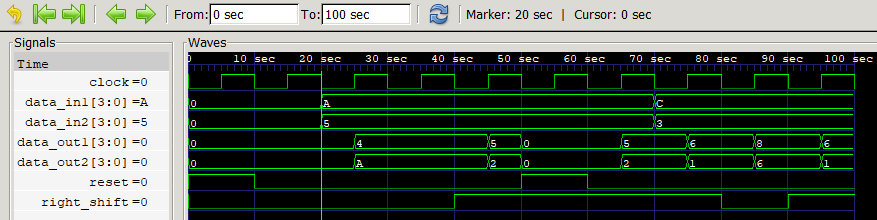
\includegraphics[width = 1.0\textwidth]{figs/Shift20.png}
    \caption{2x4-bit output Shift Circuit with marker at 20s}
    \label{fig:enter-label}
\end{figure}


At 30 s, we can see that data in1 is A and data in2 is 5, so that means that data out1 is 4 and data out2 is A
\begin{figure}[h]
    \centering
    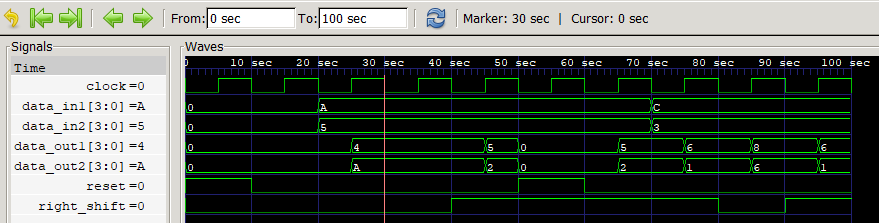
\includegraphics[width = 1.0\textwidth]{figs/Shift30.png}
    \caption{2x4-bit output Shift Circuit with marker at 30s}
    \label{fig:enter-label}
\end{figure}


At 40 s, we can see that data in1 is A and data in2 is 5, so that means that data out1 is 4 and data out2 is A
\begin{figure}[h]
    \centering
    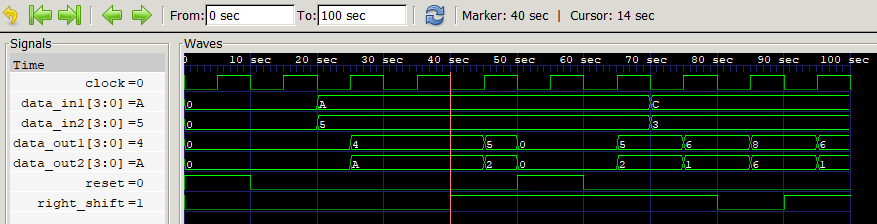
\includegraphics[width = 1.0\textwidth]{figs/Shift40.png}
    \caption{2x4-bit output Shift Circuit with marker at 40s}
    \label{fig:enter-label}
\end{figure}

\newpage

At 50 s, we can see that data in1 is A and data in2 is 5, so that means that data out1 is 0 and data out2 is 0
\begin{figure}[h]
    \centering
    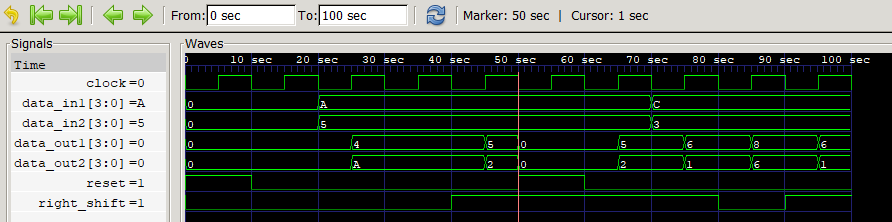
\includegraphics[width = 1.0\textwidth]{figs/Shift50.png}
    \caption{2x4-bit output Shift Circuit with marker at 50s}
    \label{fig:enter-label}
\end{figure}


At 60 s, we can see that data in1 is A and data in2 is 5, so that means that data out1 is 0 and data out2 is 0
\begin{figure}[h]
    \centering
    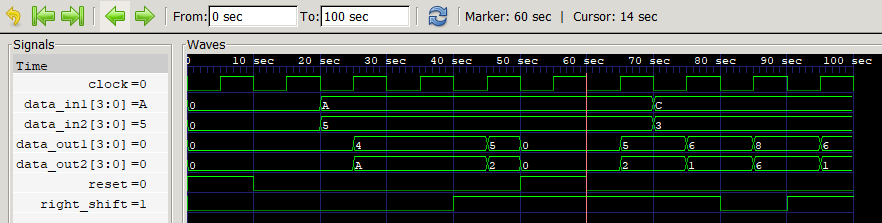
\includegraphics[width = 1.0\textwidth]{figs/Shift60.png}
    \caption{2x4-bit output Shift Circuit with marker at 60s}
    \label{fig:enter-label}
\end{figure}

At 70 s, we can see that data in1 is C and data in2 is 3, so that means that data out1 is 5 and data out2 is 2
\begin{figure}[h]
    \centering
    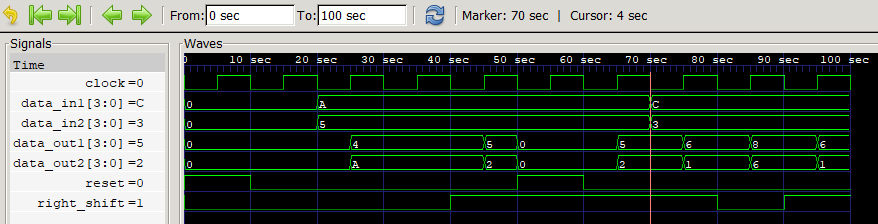
\includegraphics[width = 1.0\textwidth]{figs/Shift70.png}
    \caption{2x4-bit output Shift Circuit with marker at 70s}
    \label{fig:enter-label}
\end{figure}

\newpage

At 80 s, we can see that data in1 is C and data in2 is 3, so that means that data out1 is 6 and data out2 is 1
\begin{figure}[h]
    \centering
    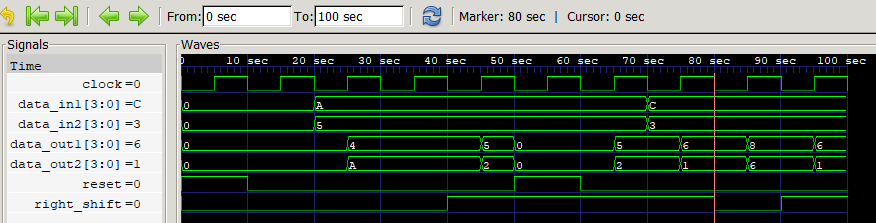
\includegraphics[width = 1.0\textwidth]{figs/Shift80.png}
    \caption{2x4-bit output Shift Circuit with marker at 80s}
    \label{fig:enter-label}
\end{figure}


At 90 s, we can see that data in1 is C and data in2 is 3, so that means that data out1 is 8 and data out2 is 6
\begin{figure}[h]
    \centering
    \includegraphics[width = 1.0\textwidth]{figs/Shift90.png}
    \caption{2x4-bit output Shift Circuit with marker at 90s}
    \label{fig:enter-label}
\end{figure}

At 100 s, we can see that data in1 is C and data in2 is 3, so that means that data out1 is 6 and data out2 is 1
\begin{figure}[h]
    \centering
    \includegraphics[width = 1.0\textwidth]{figs/Shift100.png}
    \caption{2x4-bit output Shift Circuit with marker at 100s}
    \label{fig:enter-label}
\end{figure}

\newpage


\subsection{Addition}

At 0 s, we can see that a is 0 and b is 0, so that means addition result is 00 and sum is 0
\begin{figure}[h]
    \centering
    \includegraphics[width = 1.0\textwidth]{figs/Add0.png}
    \caption{Addition Circuit with marker at 0s}
    \label{fig:enter-label}
\end{figure}

At 10 s, we can see that a is 1 and b is 1, so that means addition result is 02 and sum is 2
\begin{figure}[h]
    \centering
    \includegraphics[width = 1.0\textwidth]{figs/Add10.png}
    \caption{Addition Circuit with marker at 10s}
    \label{fig:enter-label}
\end{figure}

At 20 s, we can see that a is 2 and b is 2, so that means addition result is 04 and sum is 4 
\begin{figure}[h]
    \centering
    \includegraphics[width = 1.0\textwidth]{figs/Add20.png}
    \caption{Addition Circuit with marker at 20s}
    \label{fig:enter-label}
\end{figure}

\newpage

At 30 s, we can see that a is 3 and b is 1, so that means addition result is 04 and sum is 4
\begin{figure}[h]
    \centering
    \includegraphics[width = 1.0\textwidth]{figs/Add30.png}
    \caption{Addition Circuit with marker at 30s}
    \label{fig:enter-label}
\end{figure}



\subsection{Subtraction}

At 0 s, we can see that A is 4 and B is 2, so then the difference is 2
\begin{figure}[h]
    \centering
    \includegraphics[width = 1.0\textwidth]{figs/Sub0.png}
    \caption{Subtraction Circuit with marker at 0s}
    \label{fig:enter-label}
\end{figure}

At 10 s, we can see that A is 2 and B is 1, so then the difference is 1
\begin{figure}[h]
    \centering
    \includegraphics[width = 1.0\textwidth]{figs/Sub10.png}
    \caption{Subtraction Circuit with marker at 10s}
    \label{fig:enter-label}
\end{figure}

\newpage

At 20 s, we can see that A is 1 and B is 1, so then the difference is 0
\begin{figure}[h]
    \centering
    \includegraphics[width = 1.0\textwidth]{figs/Sub20.png}
    \caption{Subtraction Circuit with marker at 20s}
    \label{fig:enter-label}
\end{figure}

At 30 s, we can see that A is 0 and B is 1, so then the difference is F
\begin{figure}[h]
    \centering
    \includegraphics[width = 1.0\textwidth]{figs/Sub30.png}
    \caption{Subtraction Circuit with marker at 30s}
    \label{fig:enter-label}
\end{figure}



\subsection{Multiplication}

At 0 s, we can see that A is 1 and B is 2, so then the product is 02
\begin{figure}[h]
    \centering
    \includegraphics[width = 1.0\textwidth]{figs/Mult0.png}
    \caption{Multiplication Circuit with marker at 0s}
    \label{fig:enter-label}
\end{figure}

\newpage

At 10 s, we can see that A is 2 and B is 3, so then the product is 06
\begin{figure}[h]
    \centering
    \includegraphics[width = 1.0\textwidth]{figs/Mult10.png}
    \caption{Multiplication Circuit with marker at 10s}
    \label{fig:enter-label}
\end{figure}

At 20 s, we can see that A is 1 and B is 1, so then the product is 01
\begin{figure}[h]
    \centering
    \includegraphics[width = 1.0\textwidth]{figs/Mult20.png}
    \caption{Multiplication Circuit with marker at 20s}
    \label{fig:enter-label}
\end{figure}

At 30 s, we can see that A is 3 and B is 2, so then the product is 06
\begin{figure}[h]
    \centering
    \includegraphics[width = 1.0\textwidth]{figs/Mult30.png}
    \caption{Multiplication Circuit with marker at 30s}
    \label{fig:enter-label}
\end{figure}

\newpage

\subsection{Division}

At 0 s, we can see that A is 4 and B is 2, so that means that the quotient is 2 and the remainder is 0
\begin{figure}[h]
    \centering
    \includegraphics[width = 1.0\textwidth]{figs/Div0.png}
    \caption{Division Circuit with marker at 0s}
    \label{fig:enter-label}
\end{figure}

At 10 s, we can see that A is 1 and B is 1, so that means that the quotient is 1 and the remainder is 0
\begin{figure}[h]
    \centering
    \includegraphics[width = 1.0\textwidth]{figs/Div10.png}
    \caption{Division Circuit with marker at 10s}
    \label{fig:enter-label}
\end{figure}

At 20 s, we can see that A is 2 and B is 1, so that means that the quotient is 2 and the remainder is 0
\begin{figure}[h]
    \centering
    \includegraphics[width = 1.0\textwidth]{figs/Div20.png}
    \caption{Division Circuit with marker at 20s}
    \label{fig:enter-label}
\end{figure}

\newpage

At 30 s, we can see that A is 0 and B is 1, so that means that the quotient is 0 and the remainder is 0
\begin{figure}[h]
    \centering
    \includegraphics[width = 1.0\textwidth]{figs/Div30.png}
    \caption{Division Circuit with marker at 30s}
    \label{fig:enter-label}
\end{figure}

At 40 s, we can see that A is 4 and B is 0, so that means that the quotient is 0 and the remainder is 0
\begin{figure}[h]
    \centering
    \includegraphics[width = 1.0\textwidth]{figs/Div40.png}
    \caption{Division Circuit with marker at 40s}
    \label{fig:enter-label}
\end{figure}


\end{document}